\chapter{Inleiding}
\chapterpreamble

%
%
%
\section{Productomschrijving}

De \product is een set van twee cartridges waarmee SD-kaartjes uitgelezen kunnen worden op de \pkb{P2000T} of \pkb{P2000M} en programma's ingeladen kunnen worden in het geheugen. Vervolgens kunnen deze programma's opgestart worden. De \product is een datadrager die vergelijkbaar is met een cassettedeck of floppydrive en welke cassette bestanden (\cas) kan inladen en opstarten in een BASICNL omgeving. Wanneer de \pkb{P2000T} voorzien is van tenminste een 16 KiB geheugenuitbreiding kan de \pkb{P2000T} ook machinetaalbestanden (\prg) inladen in het geheugenblok \pkb{0xA000-0xDFFF} en opstarten.

%
%
%
\section{Versies}
Over de tijd zijn er verschillende aanpassingen aan \product gemaakt en heeft de printplaat meerdere iteraties doorgemaakt. Vanaf revisie 7 van de printplaat is de I/O poort waarmee de \product verbinding maakt met de printer gewijzigd van \pkb{0x60} naar \pkb{0x40} omdat sommige andere componenten ontwikkeld voor de \pc al reeds poort \pkb{0x60} gebruiken. Om die reden heeft alle software twee versies, een \pkb{0x60} en een \pkb{0x40} versie. Wanneer u een printplaat met revisie 6 (REV5) of ouder (lager nummer) gebruikt, gebruik dan de \pkb{0x60} versie van de software. Voor revisie 7 (REV6) en nieuwer, gebruik dan \pkb{0x40}. Om het verschil duidelijk aan te geven hebben alle cartridge-behuizingen vanaf REV6 op de voorzijde de indicatie \pkb{0x40} geprint. Wanneer er geen indicatie op de cartridge staat kunt u ervan uitgaan dat u een versie \pkb{0x60} cartridge heeft. Buiten de andere I/O poort zijn er voor de rest slechts minimale verschillen tussen de printplaten en zult u weinig tot geen verschil in het gebruik opmerken. Indien er desondanks relevante verschillen zijn tussen de varianten zullen deze in de handleiding opgemerkt worden met \faLocationArrow\pkb{0x60} en \faLocationArrow\pkb{0x40}.

\admonition{warning}{Let op!}{Gebruik de juiste software voor de cartridge. Indien de tekst \pkb{0x40} op de cartridge staat, gebruik dan de \pkb{0x40} variant. Staat er niets aangegeven, gebruik dan de \pkb{0x60} variant.}

%
%
\subsection{Technische specificaties}

\begin{itemize}[noitemsep]
    \item 16 MHz klok-generator
    \item 128 KiB alleen-lezen geheugen (ROM)
    \item 128 KiB schrijfbaar geheugen (RAM)
    \item \faLocationArrow\pkb{0x60}: SD-kaart houder met 5V naar 3.3V spanningsomvormer en bidirectionele niveauregelaar; \faLocationArrow\pkb{0x40} geïntegreerde SD-kaart slot en 3.3V spanningsomvormer op de hoofdprintplaat.
    \item 2 x 8-bit registers voor de adresbus van de ROM en RAM chips
    \item 1 x 2-bit register voor bankselectie van de ROM en RAM chips (2 x 64 KiB banken)
    \item 2 schuifregisters voor data-communicatie met de SD-kaart
\end{itemize}

%
%
%
\section{Cartridges}

De \product is een set van twee cartridges: een \sleuf{1} en \sleuf{2} cartridge. De \sleuf{1} cartridge heeft aan de voor- of bovenzijde een DIP schakelaar, de \sleuf{2} cartridge heeft aan de voorzijde 4 LED-lampjes\index{LED-lampjes}. Over het algemeen wordt de \sleuf{1} cartridge geleverd met een zwart-oranje behuizing en de \sleuf{2} cartridge met een zwart-witte behuizing.

\admonition{warning}{Let op!}{Er bestaan meerdere soorten multirom cartridges met een verschillende capaciteit. We bespreken hier een variant van 64 KiB, welke 4x16 KiB cartridge banken heeft. Heeft u een ZIF-variant of de 32x16 KiB variant, dan kunnen de benodigde cartridges op andere banken. Het kan ook zijn dat de cartridges nog op de multirom geschreven moeten worden. Zie voor meer informatie de bijbehorende handleiding of neem contact op met de ontwikkelaar.}

%
%
%
\subsection{Sleuf 1 cartridge}

\index{Sleuf 1 cartridge}
\index{SLOT 1 cartridge|see{Sleuf 2 cartridge}}

Cartridge 1 (zwart-oranje) is een \sleuf{1} multirom cartridge (zie \cref{fig:cartridge-sleuf1}) waarbij de gebruiker middels een DIP schakelaar aan de voorzijde van de cartridge de gewenste ROM kan selecteren.

\begin{figure}[h!]
    \centering
    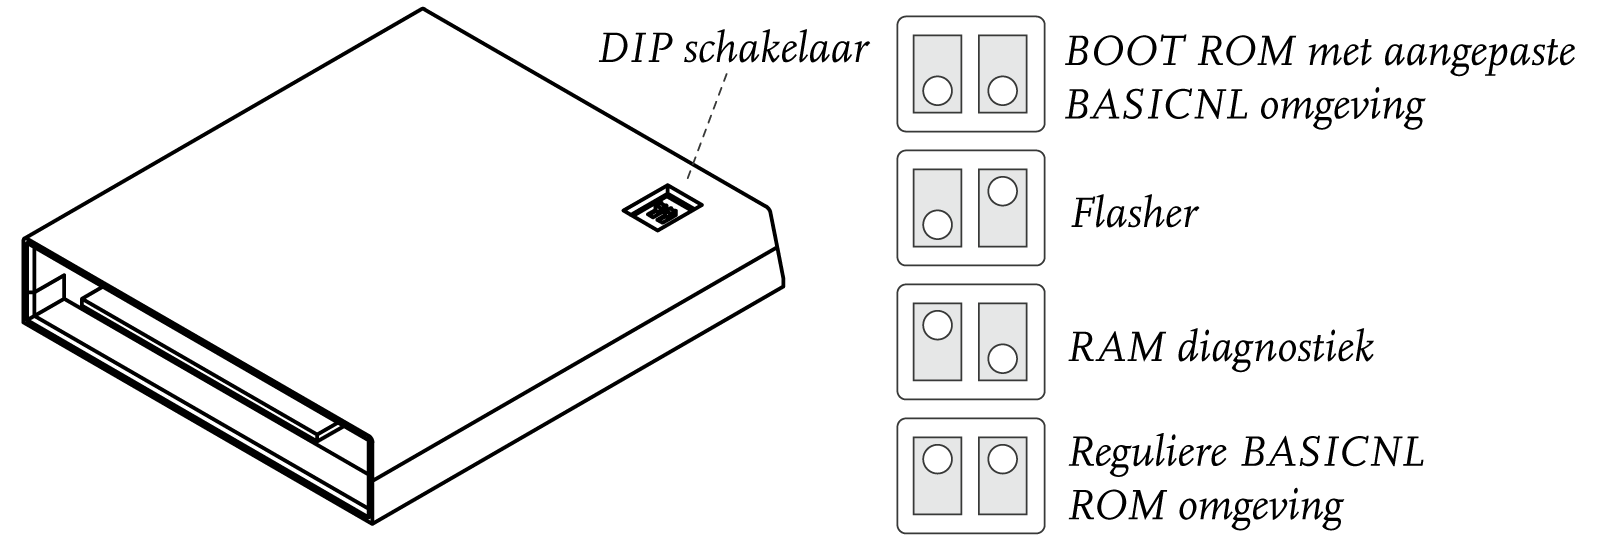
\includegraphics[width=0.99\textwidth]{img/slot1-cartridge.png}
    \caption{Sleuf 1 cartridge. Middels de DIP schakelaar kan het gewenste ROM geselecteerd worden.}
    \label{fig:cartridge-sleuf1}
\end{figure}

De cartridge bevat een 64 KiB ROM chip waardoor op deze (enkele) cartridge de inhoud van vier reguliere cartridges (4 x 16 KiB) geplaatst kan worden. De volgende cartridge-roms zijn op de \sleuf{1} cartridge aanwezig:

\begin{enumerate}[noitemsep]
    \item Aangepaste BASICNL v1.1 om cassette bestanden op te kunnen starten. (zie \cref{chap:usage})
    \item Flash programma om de firmware op Cartridge 2 (zwart-wit) te kunnen updaten. (zie \cref{sec:firmware-flash})
    \item Geheugen test om te controleren of het geheugen in de \pkb{P2000T} (inclusief eventuele geheugenuitbreidingen) correct functioneert.
    \item Kopie van de reguliere BASICNL v1.1 cartridge voor als de gebruiker de \pkb{P2000T} in de reguliere BASICNL omgeving wilt opstarten.
\end{enumerate}

\admonition{danger}{Waarschuwing!}{Verander de DIP schakelaar nooit als de \pc in bedrijf is. Dit kan de werking van de \pc verstoren. Zet altijd eerst de \pc uit voordat u een andere cartridge-rom selecteert middels de DIP schakelaar.}

%
%
%
\subsection{Sleuf 2 cartridge}

\index{Sleuf 2 cartridge}
\index{SLOT 2 cartridge|see{Sleuf 2 cartridge}}

Cartridge 2 (zwart / wit) is een \sleuf{2} cartridge (zie \cref{fig:cartridge-sleuf2}) met de benodigde schakelingen zodat de \pkb{P2000T} kan communiceren met het SD kaartje. Deze cartridge bevat naast een SD-kaart houder, ook een 128 KiB ROM chip (SST39SF010) en een 128 KiB RAM chip (62128). De ROM chip wordt gebruikt om de firmware op te slaan terwijl de RAM chip gebruikt wordt als buffer zodat grote stukken data opgeslagen kunnen worden zonder het interne geheugen van de \pkb{P2000T} te belasten.

\begin{figure}[h!]
    \centering
    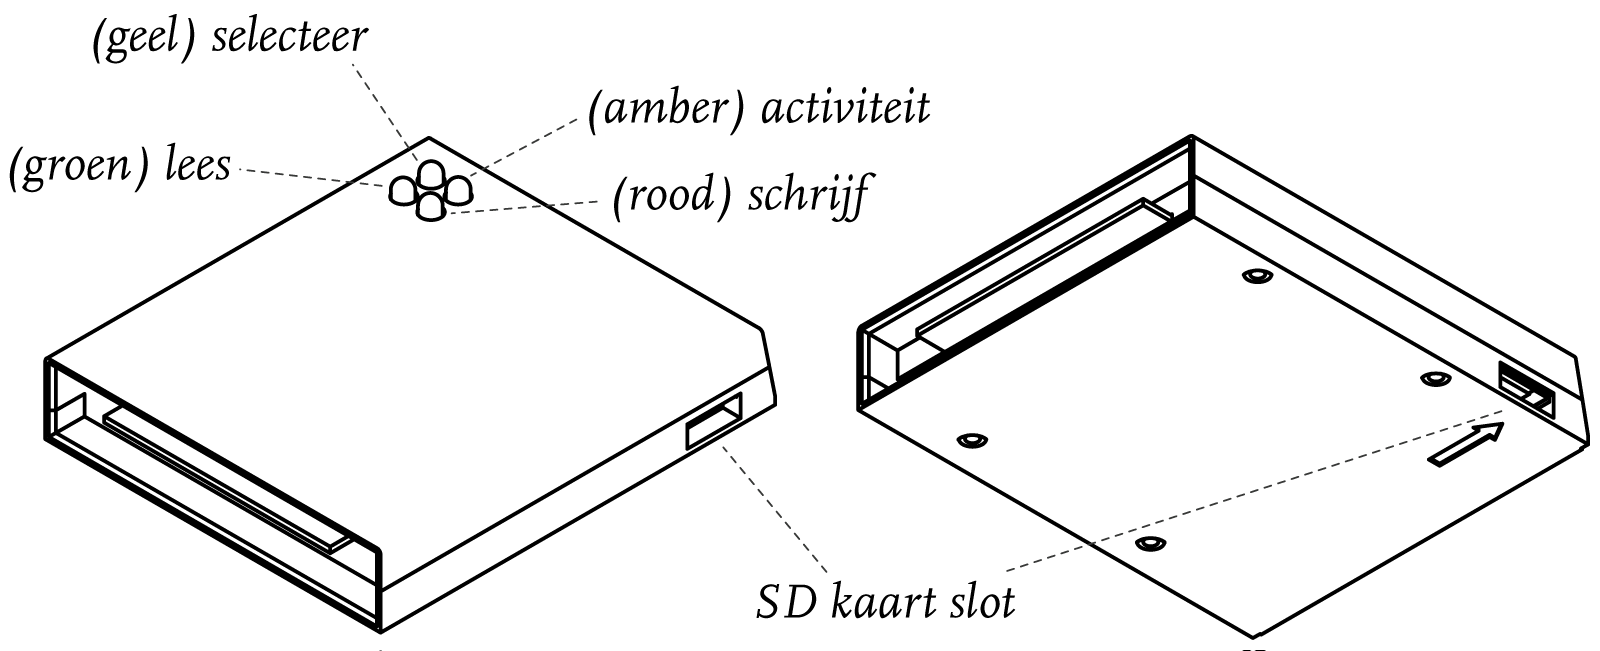
\includegraphics[width=0.99\textwidth]{img/sd-card-cartridge.png}
    \caption{Sleuf 2 cartridge. Vier LED-lampjes aan de bovenzijde (linker afbeelding) geven de operaties op de cartridge aan. Aan de onderzijde (rechter afbeelding) geeft een pijl de uitsparing voor de SD-kaart lezer aan.}
    \label{fig:cartridge-sleuf2}
\end{figure}

Aan de voorzijde van de cartridge bevinden zich 4 LED-lampjes. Deze geven de lopende operaties van de cartridge aan.

\begin{itemize}[noitemsep]
    \item \pkb{Geel}: De SD-kaart is geactiveerd.
    \item \pkb{Amber}: Er is data-overdracht tussen de SD-kaart en de \pkb{P2000T}.
    \item \pkb{Groen}: Er wordt vanaf de cartridge gelezen. Deze lees-operaties zijn naar de ROM of RAM chip.
    \item \pkb{Rood}: Er wordt data naar de cartridge geschreven. Deze schrijf-operaties zijn naar de ROM of naar de RAM chip.
\end{itemize}

%
%
%
\section{Broncode, schema's en licentie}

\index{licentie}
\index{broncode}

De \product is een volledig open-source en open-hardware product. De bronbestanden om de PCBs te fabriceren en de broncode voor de software zijn te verkrijgen via deze Github repository:\\ \faGithub \;\url{https://github.com/ifilot/p2000t-sdcard/}.

\begin{center}
    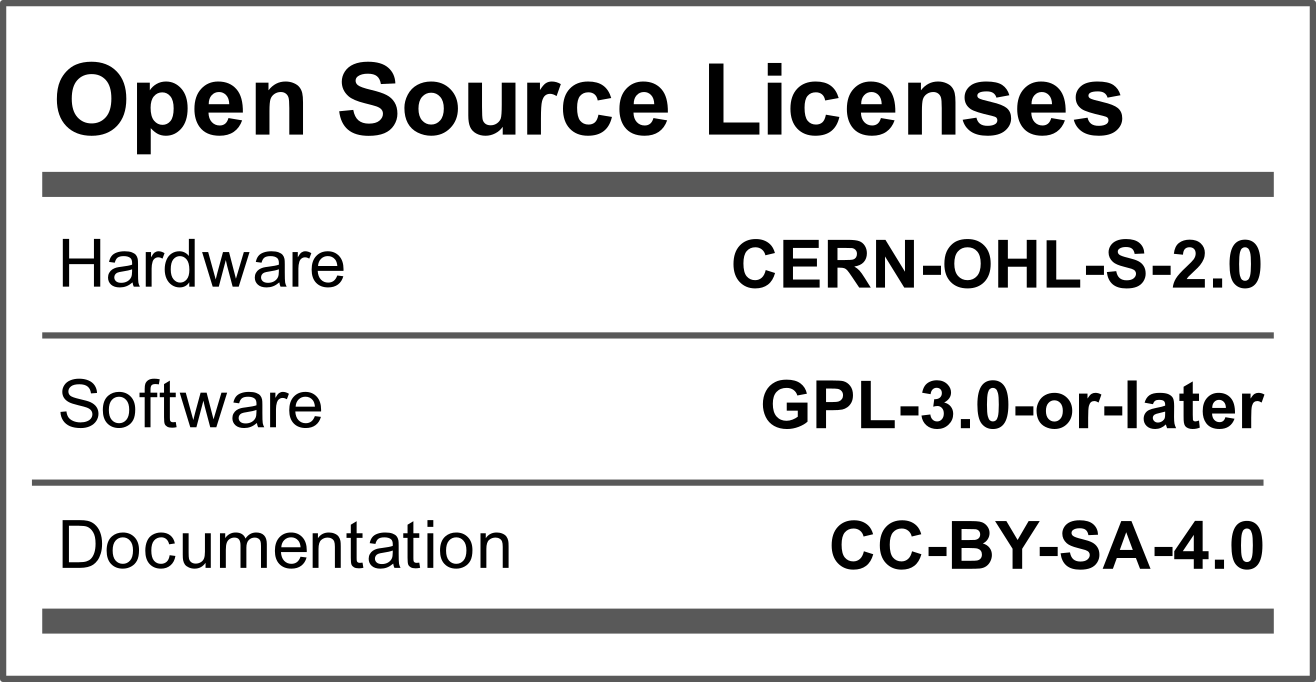
\includegraphics[width=0.5\textwidth]{img/oshw_facts.png}
\end{center}

\begin{itemize}
    \item De hardware licentie betreft CERN-OHL-S-2.0\footnote{\url{https://ohwr.org/project/cernohl/-/wikis/uploads/819d71bea3458f71fba6cf4fb0f2de6b/cern_ohl_s_v2.txt}}.
    \item De software wordt gedistribueerd onder een GPLv3\footnote{\url{https://www.gnu.org/licenses/gpl-3.0.en.html}} licentie.
    \item De documentatie valt onder een CC-BY-SA\footnote{\url{https://creativecommons.org/licenses/by-sa/4.0/deed.en}} licentie.
\end{itemize}

\newpage

De \product is geregistreerd bij de Open Source Hardware Association onder registratienummer \pkb{NL000022}.\footnote{\url{https://certification.oshwa.org/nl000022.html}}

\begin{center}
    
\includegraphics[width=0.9\textwidth]{img/certification-mark-NL000022-wide.png}
\end{center}